%--
%-- Diagrama de Contexto
%--
\subsection{Diagrama de Contexto}

%--
%-- Listado de Fenómenos
%--
\subsubsection{Listado de Fenómenos}
\begin{enumerate}
 \item Configuración y uso por parte del Administrador
  \begin{enumerate}
   \item El Administrador ingresa credenciales en el Sistema
   \item El Administrador define el umbral de redituabilidad en el Sistema
   \item El Administrador consulta estadísticas en el Sistema
  \end{enumerate}

 \item Registro presencial cliente
  \begin{enumerate}
      \item El Cliente se traslada a la Sucursal
      \item El Cliente presenta la documentación en la Sucursal
      \item El Cliente presenta la factura asociada al domicilio en la Sucursal
      \item El Cliente presenta datos de tarjeta en la Sucursal
      \item La Sucursal presenta datos de tarjeta del cliente al Agente de Cobro
      \item El Agente de Cobro verifica la tarjeta de crédito del Cliente
      \item La Sucursal verifica datos personales y de domicilio del Cliente
      \item La Sucursal carga datos del cliente en el Sistema
  \end{enumerate}
  
 \item Registro online cliente
  \begin{enumerate}
    \item El Cliente presenta datos de identificación personal y de domicilio al Sistema
    \item El Cliente presenta datos de pago al Sistema
    \item El Sistema valida domicilio con el Correo Argentino
    \item La Financiera evalúa estado financiero del Cliente
    \item El Agente de Cobro valida datos de pago del Cliente
    \item El Sistema añade al Cliente
  \end{enumerate}
  
 \item Registro pedido
  \begin{enumerate}
    \item El Cliente ingresa credenciales en el Sistema
    \item El Sistema muestra stock disponible al Cliente
    \item El Sistema muestra recomendaciones al Cliente
    \item El Cliente selecciona mercadería en el Sistema
  \end{enumerate}
 
 \item Acuerdo de fecha
  \begin{enumerate}
    \item Logística le calcula el costo de envío al domicilio al Sistema
    \item Si el cliente no recibi\'o alg\'un pedido: 
      \begin{enumerate}
      \item El Sistema bloquea contraentrega al Cliente
      \item El Sistema ofrece pago de multa para salvarlo
      \end{enumerate}
    \item El Sistema contabiliza ingresos producidos por compras del Cliente
    \item El Sistema evalúa ingreso generado por influencia social del Cliente
    \item El Sistema informa métodos de pago disponibles al Cliente
    \item EL Cliente elige forma de pago en el Sistema
    \item Si la forma de pago es online: 
    \begin{enumerate}
      \item El Cliente paga el pedido al Agente de Cobro
      \item El Agente de cobro confirma el pago al Sistema
      \item El Sistema confirma la recepción del pago al Cliente
    \end{enumerate}
  \end{enumerate}
  
 \item Modificaci\'on de pedido
  \begin{enumerate}
    \item El Cliente modifica un pedido no cerrado en el Sistema
    \item El Sistema le dá un crédito al Cliente si este quita mercadería paga
  \end{enumerate}

 \item Preparación y entrega
  \begin{enumerate}
    \item El Cliente confirma el pedido al Sistema
    \item El Sistema avisa al Depósito que prepare el pedido 
    \item El Depósito informa egreso de mercadería al Departamento de stock
    \item El Depósito avisa al Sistema que el pedido está cerrado
    \item El Depósito entrega mercadería a Logística
    \item Si forma de pago es contraentrega: 
    \begin{enumerate}
      \item Cliente paga el pedido a Logística
    \end{enumerate}
    \item Logística entrega el pedido al Cliente
    \item El Sistema actualiza positivamente el perfil del Cliente
  \end{enumerate}

 \item Entrega fallida
  \begin{enumerate}
    \item El Cliente no recibe pedido a Logística
    \item El Sistema reintegra el dinero al Cliente si este no lo recibe
    \item El Sistema añade una no-recepción al historial de recepciones del Cliente
    \item Logística devuelve el stock al Depósito
    \item El Sistema de Correo electrónico ofrece rehacer el pedido Cliente
  \end{enumerate}

 \item Reposicion stock sucursal
  \begin{enumerate}
    \item La Sucursal avisa cuando falta stock al Sistema
    \item El Sistema avisa falta de stock en sucursal al Depósito
    \item El Depósito arma pedido y entrega el stock a Logística
    \item El Sistema disminuye stock en el Depósito
    \item Logística entrega stock a la Sucursal
  \end{enumerate}

 \item Reposicion stock deposito
  \begin{enumerate}
    \item El Departamento de stock modifica los límite m\'inimos de stock estipulado para cada producto en el Sistema
    \item El Sistema avisa que hay faltante de producto al Departamento de stock
    \item El Departamento de stock encarga reposición de stock del depósito a Logística
    \item Logística repone stock al Depósito
  \end{enumerate}

 \item Cierre de sesi\'on
  \begin{enumerate}
    \item Cliente cierra sesión en el Sistema
    \item Administrador	cierra sesión en el Sistema
  \end{enumerate}
\end{enumerate}


%--
%-- Agentes
%--
\subsubsection{Agentes}

\begin{enumerate}
  \item Depósito
  \item Cliente
  \item Sucursal
  \item Sistema
  \item Logística
  \item Departamento de stock 
  \item Agente de Cobro
  \item Administrador
  \item Sistema de Correo Electrónico
  \item Financiera\footnote{Ejemplo: VERAZ}
  \item Correo Argentino
\end{enumerate}

%--
%-- Acciones Básicas
%--
\subsubsection{Diagrama de Contexto}

\begin{figure}[H]
  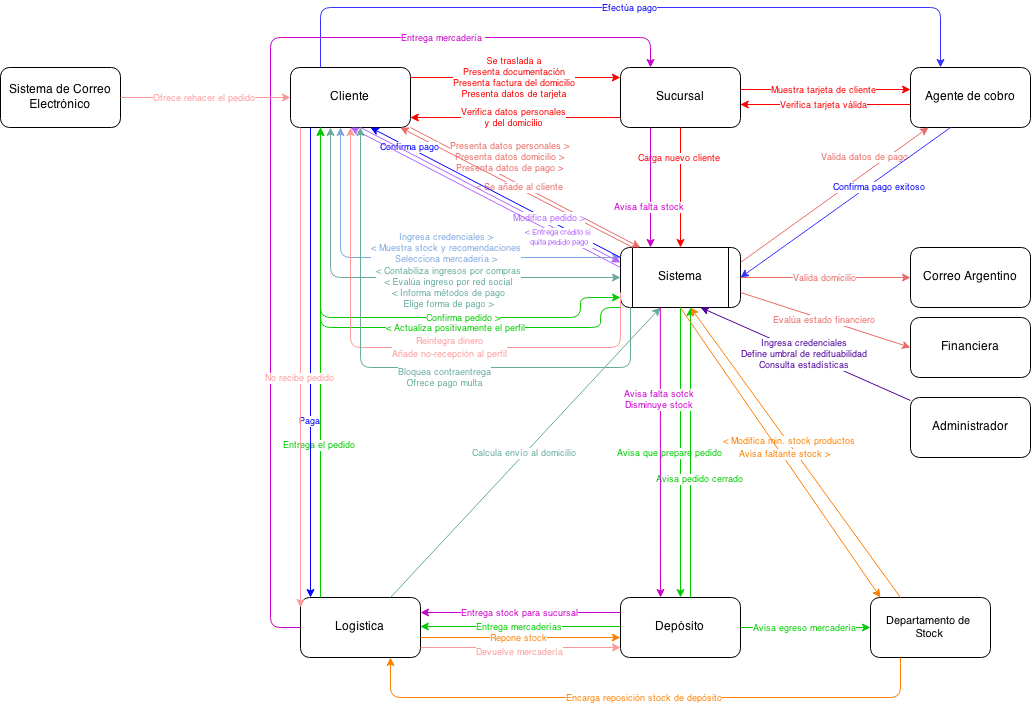
\includegraphics[width=\linewidth]{images/contexto.png}
\end{figure}
